% this file is called up by thesis.tex
% content in this file will be fed into the main document
\ifpdf
    \graphicspath{{3/figures/PNG/}{3/figures/PDF/}{3/figures/}}
\else
    \graphicspath{{3/figures/EPS/}{3/figures/}}
\fi
\chapter{Technologie} % top level followed by section, subsection


% ----------------------- contents from here ------------------------
W rozdziale tym, zostaną zaprezentowane oraz po krótce opisane najważniejsze technologie wykorzystane przy implementacji przykładowego systemu  powstałego na bazie tej pracy.

\section{OSGi}
Technologia OSGi to zbiór specyfikacji definiujących dynamiczne środowisko komponentowe. Taka struktura pozwala na tworzenie aplikacji złożonych z wielu, różnych komponentów(bundle) które mogą być wykorzystywane wiele razy. Specyfikacja OSGi umożliwia bundle'om ukrywanie swojej implementacji przed innymi komponentami i komunikację tylko przy użyciu specjalnych serwisów, które są dzielone pomiędzy bundle'ami. Pozwala to na zmniejszenie złożoności tworzonych systemów.

OSGi posiada architekturę warstwową, przedstawiona jest ona, wraz z krótkim opisem, na poniższym diagramie.
\newpage
\begin{figure}[!h]
	\centering
	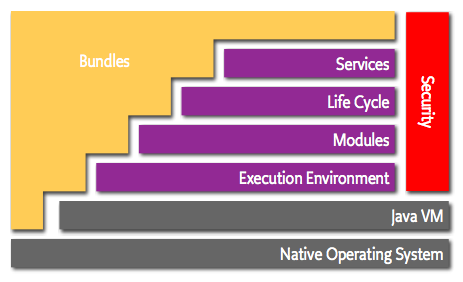
\includegraphics[scale=0.65]{osgiArchitektura.png} 
	\caption{Architektura OSGi}
\end{figure}
\begin{itemize}
	\item Bundles - Są to OSGi'owe, mogą być preinstalowane jak i tworzone i dynamicznie ładowane przez programistów
	\item Services - Warstwa serwisów dynamicznie łączy komponenty, stosując model publish-find-bin
	\item Life-Cycle - API do startowania, zatrzymywania, instalowania i dezinstalowania komponentów
	\item Modules - Warstwa definiująca jak komponenty mogą importować i eksportować kod	
	\item Security - Warstwa zajmująca się bezpieczeństwem
	\item Execution Environment - Warstwa definiująca jakie metody i klasy są dostępne na specyficznej plarformie
\end{itemize}  
Najważniejszym konceptem umożliwiającym istnienie i działanie takiej platformy jest modułowość, której ucieleśnieniem są bundle. OSGi ukrywa wszystko co znajduje się w takim komponencie poza funkcjonalnością która jest wyspecyfikowana. Jeżeli jeden komponent chce wykorzystać inny musi wyraźnie definiować jaką funkcjonalność potrzebuje. Ponieważ ciężko stworzyć model współpracy opierając się tylko na klasach OSGi wprowadza wastwę serwisów, a wraz z nią rejestr serwisów. Bundle może stworzyć obiekt i zarejestrować go w rejestrze pod jednym lub więcej interfejsów. Inne komponenty mogą z takiego rejestru pobierać obiekty stosując różne kryteria, na przykład wszystkie obiekty implementujące dany interfejs itd.
\begin{figure}[!h]
	\centering
	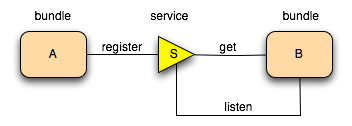
\includegraphics[scale=0.75]{serveLayer.png} 
	\caption{Zalezność pomiędzy bundlami i serwisami}
\end{figure}
 Możliwe jest oczywiście, żeby dowolna liczba komponentów zarejestrowała ten sam typ serwisów lub też pobrała ten sam serwis. Oczywiście zarejestrowane serwisy można rozróżniać, każdy ma powiązany ze sobą zestaw właściwości(properties), które mogą służyć do specyfikacji. Cała warstwa serwisów jest dynamiczna, bundle mogą dodawać, usuwać itd. serwisy bez konieczności restartu kontenera.  \\
Do tworzenia i definiowana zależności między bundlami OSGi wykorzystuje Blueprint Container. Jest to framework którego celem jest zarządzanie wstrzykiwaniem zależności. Został zaprojektowany żeby radzić sobie z dynamiczną specyfikacją OSGi'a (możliwość pojawienia się i zniknięcia serwisów w dowolnym momencie). Jego specyfikacja pozwala mu też na działania w środowisku innym niż OSGi'owe. W założeniu opiera się on o strukturę plików xml, które definiują jak komponenty są tworzone oraz łączone aby stworzyć działającą aplikację. Sposób działania kontera opiera się o wzorzec Extender. W czasie inicjalizacji bundle'a (a więc w czasie działania kontenera) Blueprint Container sprawdza czy wszystkie wymagane zależności są spełnione, tworzy wszystkie wymagane obiekty oraz rejestruje serwisy. 

\section{SOA}
SOA czyli Service Oriented Architecture(Architektura zorientowana na usługi) to zgodnie z definicją zaproponowaną przez W3C to zbiór komponentów dostępnych w siecii posiadających dobrze opisane interfejsy. Opis ten pozwala na rozróżnianie komponentów i ich wyszukiwanie, a następnie wywoływanie. Najbardziej popularną obecnie implementacją tego paradygmatu jest ta opierająca się o web serwisy.  W paradygmacie SOA możemy wyróżnić dwa różne podejścia tworzenia serwisów:
 \begin{itemize}
	\item orkiestracja
	\item choreografia
\end{itemize}  
Orkiestracja charakteryzuje się tym, iż istnieje jeden serwis orkiestrator, dyrygent lub kordynator który zarządza innymi serwisami w celu udostępniania jednej funkcjonalności. Prowadzi to do luźniejszego połączenia serwisów, sprawia też, że nie są one świadome bycia częścią większego procesu. Orkiestracja jest scentralizowaną formą współpracy z dobrze zdefiniowanymi operacjami i kolejnością wywoływania serwisów. Powstał nawet specjalny język BPEL ułatwiający taką integrację serwisów.   
\begin{figure}[!h]
	\centering
	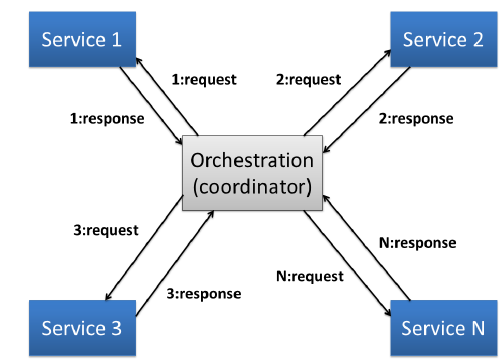
\includegraphics[scale=0.75]{orkiestracja.png} 
	\caption{Orkiestracja}
\end{figure}
\newpage
Choreografia to sposób współpracy serwisów, charakteryzujący się tym,  iż każdy serwis musi być świadomy bycia częścią czegoś większego, od niego zależy kiedy i z kim się skomunikuje. Nie ma tutaj centralnego zarządzania, kordynatora czy też serwisu nadrzędnego. Stworzenie alternatywnego scenariusza w przypadku awarii jest ciężkie albo wręcz niemożliwe. 
\begin{figure}[!h]
	\centering
	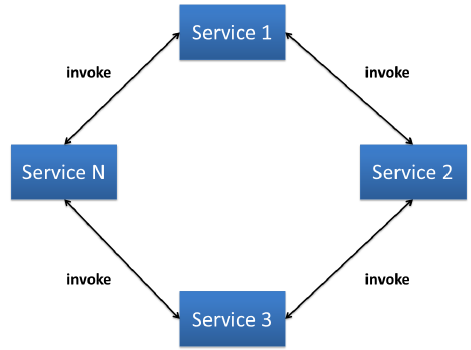
\includegraphics[scale=0.75]{choreogragia.png} 
	\caption{Choreografia}
\end{figure}

\section{Web serwisy}
Web  serwis to system zaprojektowany do wspierania komunikacji między róznymi komputerami za pomocą sieci.  Podstawowe cechyb web serwisu to:
\begin{itemize}
	\item jest komponentem mogącym być osadzonym w innej aplikacji
	\item komunikacja przy użyciu otwartych protokołów
	\item jest samodzielny i samo-opisujący się
	\item może być zlokalizowany za pomocą UDDI
	\item jest wykorzystywany przez inne aplikacje
\end{itemize}  
Można rożróżnić 2 główne klasy web serwisów:
\begin{itemize}
	\item web serwisy zgodne z architekturą REST'ową
	\item web serwisy z których każdy może udostępniać dowolny zbiór operacji
\end{itemize}  
Serwisy z grupy pierwszej \cite{fielding2000} ograniczają swój interfejs do zbioru dobrze znanych i wspieranych przez protokół transportowy operacji takich jak: PUT, GET, POST itd. dla  HTTP. Nacisk jest tutaj skierowany na interakcję z zasobami bezstanowymi. Koncpecja serwisów REST'owych opiera się na szcześciu kluczowych punktach:
\begin{itemize}
	\item model klient-serwer - wprowadza rozdzielenie odpowiedzialności, oznacza to, że na przykład klient nie interesuje się przechowywaniem danych, jest to sprawa wewnętrznej implementacji serwera, a serwer nie interesuje się interfejsem użytkownika co wprowadza prostotę i zwiększa skalowalność
	\item bezstanowość - kontekst aplikacji klienckiej nie jest przechowywany na serwerze pomiędzy zapytaniami, każde nowe zapytanie zawiera wszystkie potrzebne informacje żeby mogło zostać obsłużone
	\item możliwość cache'owania - aplikacje klienckie mogą cache'ować odpowiedzi, wymaga to od serwera by odpowiedź była pośrednio lub bezpośrednio zdefiniowana jako możliwa do cache'owania lub nie, poprawne zarządzanie tą cechą może w sposób znaczy ograniczyć komunikację na linii klient-serwer
	\item warstwowy system - klient nie jest w stanie stwierdzić czy jest bezpośrednio podpięty do serwisy czy po drodze znajdują sie inne serwisy, takie jak na przykład load-balancer
	\item opcjonalnie wykonanie kodu na rządanie - możliwe jest żeby serwer wykonał kod przesłany przez klienta
	\item jednolity interfejs - upraszcza oraz rozluźnia powiązanie między klientem a serwerem, dzięki temu możliwa jest ich niezależna ewolucja
\end{itemize}   
Serwisy z grupy drugiej reprezentują bardziej klasyczne podejście. Do opisania swoich interfejsów mogą (nie jest to wymagane jednak bardzo popularne, co więcej konieczne jeżeli chce się użyć framework'ku do generowania kodu) wykorzystywać WSDL. Jest to skrót od Web Service Description Language, formacie bazującym na XML, wykorzystywanym do opisywania jak wywołać dany serwis, jakie parametry wejściowe przyjmuje i jakie struktury danych zwraca. Inne systemy mogą komunikować się z web serwisem za pomocą protokułu SOAP. Skrót pochodzi od angielskiej nazyw Simple Object Access Protocol. Dostarcza on standardowy, rozszerzalny, dobrze zdefiniowany fremwork do wymiany wiadomości XML. Wspiera kilka różnych protokołów transportowych takich jak:
 \begin{itemize}
	\item HTTP
	\item SMTP
	\item FTP
	\item RMI/IIOP
\end{itemize}  
\begin{figure}[!h]
	\centering
	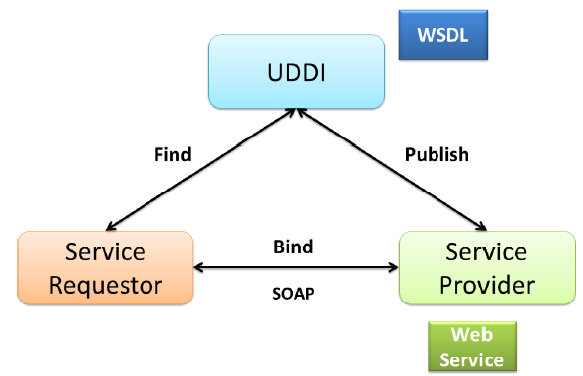
\includegraphics[scale=0.75]{webSerwisyArchitektura.png} 
	\caption{Architektura web serwisów w podejściu klasycznym}
\end{figure}

\section{Apache ServiceMix}
Apache ServiceMix pomaga rozwiązać problem integracji będąc bazującym na standardach, lekkim oraz stosującym paradygmat "luźnego powiązania" narzędziem. Dzięki bazowaniu na standardach w sposób znaczący zmniejsza szanse na uzależnienie się od konkretnego dostawcy oprogramowania, przez stosowanie luźnego powiązania pomiędzy poszczegolymi komponentami zmniejsza złożoność integracji. Jest to otwarta implementacja ESB, zbudowana w oparciu o JBI i wydana na licencji Apache, od wersji 4 ServiceMix wykorzystuje OSGi do uproszczenia podziału aplikacji na komponenty. 	
Architekturę ServiceMix'a można podzielić na 3 warstwy:
\begin{enumerate}
	\item Warstwa jądra
	\item Warstwa serwisów
	\item Warstwa aplikacji
\end{enumerate}  
\begin{figure}[!h]
	\centering
	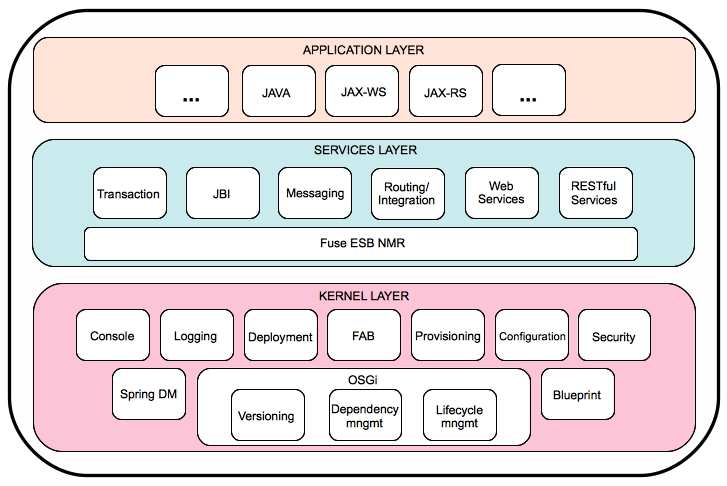
\includegraphics[scale=0.45]{ServiceMixArchitektura.jpg} 
	\caption{Architektura ServiceMix 4}
\end{figure}
Każda z tych warstw ma inne zadania i odpowiada za inne czynności.
\begin{itemize}
	\item Warstwa jądra - bazuje na Apache Karaf czyli implementacji OSGi będącą lekkim kontenerem w którym można osadzić różne komponenty i aplikacje. Warstwa ta wspólpracuje z warstwą serwisów w celu stworzenia, skoordynowania, utrzymania i zarządzania logowaniem, bezpieczeństwem oraz transakcjami. Najważniejsze funkcje dostarczane przez tą warstwę to:
	\begin{itemize}
		\item Osadzanie - umożliwia zarówno manualne jak i automatyczne osadzanie bibliotek
		\item Kontener OSGi - ServiceMix 4 wspiera 2 różne kontenery OSGi a mianowicie Eclipse Equinox i Apache Felix
		\item Wstrzykiwanie zależnośći - wykorzystuje 2 różne frameworki:
			\begin{itemize}
				\item Blueprint
				\item Spring DI
			\end{itemize}   
		\item Automatyczna konfiguracja - dokonując zmian w pliku z właściwościami można dokonać zmian "w locie", bez restartowania serwera
		\item Bezpieczeństwo - framework odpowiadający za bezpieczeństwo bazuje na JAAS, dostarcza kilka różnych, odizolowanych poziomów:
			\begin{itemize}
				\item kontenera OSGi
				\item wbudowanej instancja serwisu wiadomości
				\item osadzonych instancji serwisow router'a i integracyjnego
			\end{itemize} 
		\item Logowanie - dynamiczne logowanie wspierające różne interfejsy takie jak: JCL, SLF4J, Avalon, łatwo konfigurowalne poprzez pliki z właściwościami
		\item Konsola - umożliwia zarządzanie i pełną kontrolę nad cała aplikacją
	\end{itemize}  
	\item Warstwa serwisów - 	składa się z interfejsów i klas reprezentujących wbudowane serwisy. Współpracuje z warstwą aplikacji w celu komunikacji z aplikacjami użytkowników które chcą korzystać z oferowanych serwisów. Najważniejsze funkcje dostarczane przez tą warstwę to:
	\begin{itemize}
		\item Rutowanie i integracja - bazuje na Apache Camel, umożliwia zdefiniowanie ścieżek i zaimplementowanie biznesowych wzorców w celach integracji a następnie osadzenie jako paczka OSGi
		\item Tworzenie serwisów webowych - bazzuje na Apache CXF, umożliwia, w prosty sposób, tworzenie i osadzanie jako paczka OSGi serwisów webowych implementujących API JAX-WS 
		\item Tworzenie serwisów zgodnych ze wzorcem REST - bazuje na Apache CXF, umożliwia w prosty sposób, tworzenie i osadazanie jako paczka OSGi serwisów zgodnych z REST implementujących API JAX-RS
		\item Tworzenie i osadzanie jednostek i zespołów serwisów bazujących na JBI
		\item Komunikacje - udostępnia serwis wiadomości w całości zbudowany na Apache ActiveMQ, umożliwiający tworzenie i osadzanie zarówno klientów jak i nadawców wiadomości JMS
		\item Menadżer transakcji - bazuje na Apache Aries, wystawia interfejs transakcji jako serwis, umożliwia tworzenie i osadzanie zarówno aplikacji bazujących na framework'u JTA jak i na Spring'u
		\item Znormalizowany ruter wiadomości - jego główną rolą jest przekazywanie wiadomości pomiędzy różnymi aplikacjami osadzonymi w kontenerze OSGi oraz, jeżeli zachodzi taka konieczność, pomiędzy aplikacjami z OSGi a aplikacjami osadzonymi w kontenerze JBI
	\end{itemize}
	\item Warstwa aplikacji - w tym miejscu znajdując się aplikacje użytkownika, ServiceMix 4 dostarcza wielu różnych API(częściowo wymienionych w warstwie serwisów) za pomocą których aplikacje klienckie mogą łączyć się i korzystać z usług oferowanych przez serwisy działające wewnątrz kontenera
\end{itemize}

\section{Apache Camel}
Apache Came\cite{ibsen2010} \cite{camel} to framework używany na szeroką skalę w systemach których celem jest rozwiązywanie problemu integracji, na przykład w ServiceMixie. Najważniejszą funkcjonalnością Camel'a jest mechanizm routingu. W celu lepszego zrozumienia sposobu działania tego framework'u należy wyjaśnić kilka pojęć:
\begin{itemize}
	\item Endpoint - implementacja wzorca Message Endpoint \cite{hohpe2003}, może odnosić się do adresu lub do serwisu znajdującego się pod tym adresem (np. źródło RSS, serwer FTP), pozwala wysyłać i odbierać wiadomości  
	\item Komponent - fabryki endpoint'ów, pozwalają w elegancki sposób tworzyć endpoint'y preferowanego typu na przykład WS, JMS, RSS itd.
	\item Procesor - konsument lub translator wiadomości, może wykonać logike biznesową lub też wywołać jakiś serwis
	\item Wiadomość - wiadomość Camel'owa
	\item Ścieżka - trasa jaką pokonuje wiadomość, zaczyna się w endpoint (producent), następnie przechodzi przez procesory(konsumenci) i opcjonalnie może zostać skierowana do innego endpoint'u 
	\item CamelContext - kontekst Camel'a, miejsce w którym komponenty, endpoint'y i procesory są zdefiniowane oraz są utworzone ścieżki z ich wykorzystaniem
\end{itemize}  
Korzystając z wszystkich wymienionych wyżej elementów Camel daje możliwość stworzenia bardzo skomplikowanego systemu złożonego z wielu różnych elementów. Za jego pomocą można łatwo zaimplementować system który pobierze plik graficzny z serwera FTP, skieruje go do serwisu OCR, następnie tak otrzymany tekst skieruje do serwisu TTS. Różnych scenariuszy może być dużo i wszystkie one są łatwe do implementacji z wykorzystaniem Camel'a. Umożliwia on dwa różne sposoby definiowania ścieżek, za pomocą pliku XML i za pomocą DSL bazującego na Javi'e.
\begin{figure}[!h]
	\centering
	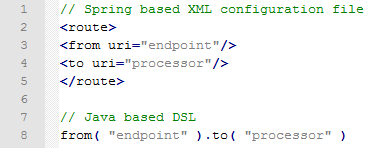
\includegraphics[scale=0.95]{camel.png} 
	\caption{Sposób definiowania ścieżek w Camel'u}
\end{figure}
			
\section{FreeTTS}
FreeTTS jest syntezatorem mowy, dostępnym na licencji opensource, w całości napisanym w języku Java. Bazuje na silniku Flite stworznym i rozwijanym przez Carnegie Mellon University. Mimo swojej prostoty jego zaletami są duża wydajność, bardzo dobre radzenie sobie z językiem angielskim oraz częściowe wsparcie dla JSAPI 1.0(jako, że jest to syntezator nie wspiera częsci specyfikacji odpowiedzialnej za rozpoznawanie mowy). Dzięki temu ostatniemu w łatwy sposób umożliwia integrację z różnymi, wieloplatformowymi aplikacjami działającymi wewnątrz JVM. Przy opisywaniu tego syntezatora istotną kwestią jest fakt, że posiada dość dobrą dokumentację oraz liczne, łatwe do uruchomienia i, co bardzo ważne, działające dema. Standardowo oferuje 3 różne głosy, wszystkie w języku angielskim, umożliwia jednak rozszerzenie liczby głosów poprzez import nowych stworzonych przy pomocy narzedzi takich jak:
\begin{itemize}
	\item FestVox,
	\item MBROLA,
	\item CMU Arctic.
\end{itemize}    

\section{Ivona TTS}
IVONA TTS to wielojęzyczny syntetyzator mowy działający w oparciu o metodę alofoniczną. Autorski algorytm stosowany przez Ivona nazywa się Bright Voices,  powstał i został opisany podczas Blizzard Challenge 2006. W chwili obecnej funkcjonalność Ivona jest dostępna na dwa sposoby:
\begin{itemize}
	\item poprzez Ivona SDK
	\item poprzez Speech Cloud (SaaS)
\end{itemize}
Ivona SDK to podstawowy sposób korzystania z usług tego oprogramowania. Dostępne są wersję na wiele różnych platform takich jak:
\begin{itemize}
	\item Linux
	\item Windows
	\item iOS
	\item Solaris
\end{itemize}
oraz w kilku różnych językach programowania:
\begin{itemize}
	\item C/C++
	\item Java
	\item ObjectiveC
	\item platforma .NET
\end{itemize}
Dostęp do Speech Cloud'a możliwy jest zarówno za pomocą protokołu SOAP oraz przez reprezentację REST'ową. W tej chwili niezależnie od używanego API można uzyskać następującą funkcjonalność:
\begin{itemize}
	\item wygenerowanie pliku dźwiękowego z podanego tekstu
	\item pobranie informacji o dostępnych głosach i kodekach
	\item zmodyfikowanie zasad wymowy, w celu poprawienia jakości wymowy niektórych słów
\end{itemize}
Syntezator ten wspiera bardzo dużo języków między innymi:
 \begin{itemize}
	\item polski
	\item angielski
	\item francuski
	\item portugalski
	\item niemiecki
\end{itemize}
Poza wyborem języka istnieje też możliwość wyboru lektora, różnią się oni barwą i siłą głosu, czy też szybkością mówienia. Możliwa jest też dynamiczna zmiana zarówno języka jak i lektora. Kolejną ważną cechą Ivona jest fakt, iż nie ogranicza się ona do jednego kodeka, wspiera następujące formaty:
\begin{itemize}
	\item mp3/22050
	\item ogg/22050
	\item pcm16/22050
	\item alaw/8000
\end{itemize}
 Aby korzystać ze zdalnego API należy posiadać konto w systemie Ivony, jest ono wykorzystywane do pobierania opłat. Co bardzo istnotne, Ivona wspiera protokół SSML, umożliwiający klientowi dokładniejsze sterowanie generowanym głosem. 

\section{Google Translate}
Google Translate to płatna usługa Google'a umożliwiająca tłumaczenie tekstu pomiędzy tysiącami dostępnych par języków. Poza tłumaczeniem usługa ta umożliwia również rozpoznanie języka. API udostępniane przez korporację opiera się o architekturę REST, składa się z trzech metod:
\begin{itemize}
	\item translate - tłumaczy tekst z języka źródłowego na docelowy, przykład:
		\begin{figure}[!h]
			\centering
			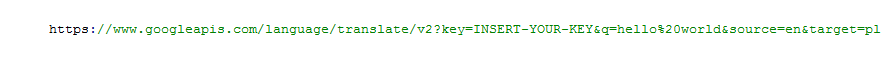
\includegraphics[scale=0.95]{translateExp.png} 
			\caption{Tłumaczenie słowa hello z angielskiego na polski}
		\end{figure}
	\item languages - zwraca listę języków wspieranych przez translator
		\begin{figure}[!h]
			\centering
			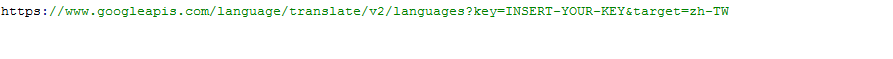
\includegraphics[scale=0.95]{listExp.png} 
			\caption{Przykład pobrania listy dostępnych języków}
		\end{figure}
	\item detect - rozpoznaje język tekstu źródłowego
		\begin{figure}[!h]
			\centering
			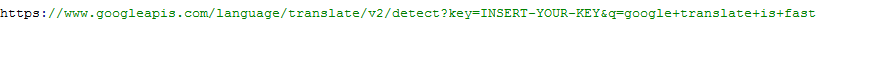
\includegraphics[scale=0.95]{detectExp.png} 
			\caption{Przykład detekcji języka}
		\end{figure}
\end{itemize}
Parametr key=INSERT-YOUR-KEY służy korporacji do indentyfikowania usługobiorcy, na jego podstawie naliczane są opłaty. Jak widać REST w API Google Translate różni się nieznacznie od tradycyjnego pojmowania tej architektury. Zamiast dostarczać dostęp do zasobów, dostarczarczany jest dostęp do usług, stosując takie podejście uzyskano możliwość wykorzystania jednego URI jako całego API. 

\section{OCR Web Service}
OCR Web Service jest to jeden z najpopularniejszych web serwisów tego rodzaju. Rozpoznaje aż dwadzieścia osiem języków między innymi:
\begin{itemize}
	\item polski
	\item angielski
	\item niemiecki
	\item francuski
	\item portugalski
\end{itemize}
Przyjmuje różne formaty wejściowe, takie jak:
\begin{itemize}
	\item JPEG\\JPG
	\item BMP
	\item PCX
	\item GIF
	\item PNG
	\item PDF
\end{itemize}
Co więcej pozwala na przekonwertowanie rozpoznanego tekstu na aż sześć różnych formatów:
\begin{itemize}
	\item Adobe PDF
	\item MS Word 2003
	\item MS Excel 2003
	\item HTML
	\item RTF
\end{itemize}
Oczywiście istnieje też możliwość otrzymania zwykłego pliku txt. Wymagania tego serwisu co do jakości obrazu w pliku otrzymanym na wejściu też nie są duże, zaleca się aby rozdzielczość wynosiła między 200 a 400 dpi. Web serwis ten jako protokół komunikacyjny wykorzystuje SOAP w wersji 1.1 lub 1.2. WSDL potrzebny do wygenerowania szkieletu kodu można pobrać ze strony projektu. Jedną z niewielu wad tego serwisu jest to, że podobnie jak Google Translate jest płatny. 